\documentclass[a4paper,17pt]{extarticle}


    \usepackage[sfdefault, condensed]{roboto} % police d'écriture plus moderne
\usepackage[french]{babel} % francisation
\usepackage[parfill]{parskip} %suppression indentation

\usepackage{fancyhdr}
\usepackage{multicol}

% figure non flotantes
\usepackage{float}
\let\origfigure\figure
\let\endorigfigure\endfigure
\renewenvironment{figure}[1][2] {
    \expandafter\origfigure\expandafter[H]
} {
    \endorigfigure
}

% mois/année
\usepackage{datetime}
\newdateformat{monthyeardate}{%
  \monthname[\THEMONTH] \THEYEAR}

% couleurs perso
\usepackage[table]{xcolor}
\definecolor{deepblue}{rgb}{0.3,0.3,0.8}
\definecolor{darkblue}{rgb}{0,0,0.3}
\definecolor{deepred}{rgb}{0.6,0,0}
\definecolor{iremred}{RGB}{204,35,50}
\definecolor{deepgreen}{rgb}{0,0.6,0}
\definecolor{backcolor}{rgb}{0.98,0.95,0.95}
\definecolor{grisClair}{rgb}{0.95,0.95,0.95}
\definecolor{orangeamu}{RGB}{250,178,11}
\definecolor{noiramu}{RGB}{35,31,32}
\definecolor{bleuamu}{RGB}{20,118,198}
\definecolor{bleuamudark}{RGB}{15,90,150}
\definecolor{cyanamu}{RGB}{77,198,244}


\usepackage{/home/bouscadilla/Documents/Code/nbconvert/template/latex/pdf_solution/xeboiboites}
%
% exemple
\newbreakabletheorem[
    small box style={fill=deepblue!90,draw=deepblue!15, rounded corners,line width=1pt},%
    big box style={fill=deepblue!5,draw=deepblue!15,thick,rounded corners,line width=1pt},%
    headfont={\color{white}\bfseries}
        ]{exemple}{Exemple}{}%{counterCo}
%
% remarque
\newbreakabletheorem[
    small box style={draw=ansi-green-intense!100,line width=2pt,fill=ansi-green-intense!0,rounded corners,decoration=penciline, decorate},%
	big box style={color=ansi-green-intense!90,fill=ansi-green-intense!10,thick,decoration={penciline},decorate},
    broken edges={draw=ansi-green-intense!90,thick,fill=orange!20!black!5, decoration={random steps, segment length=.5cm,amplitude=1.3mm},decorate},%
    other edges={decoration=penciline,decorate,thick},%
    headfont={\color{ansi-green-intense}\large\scshape\bfseries}
    ]{remarque}{Remarque}{}%{counterCa}
%
% formule (sans titre)
\newboxedequation[%
    big box style={fill=cyanamu!10,draw=cyanamu!100,thick,decoration=penciline,decorate}]%
    {form}
%
% Réponse
\newbreakabletheorem[
    small box style={fill=bleuamu!100, draw=bleuamu!60, line width=1pt,rounded corners,decorate},%
    big box style={fill=bleuamu!10,draw=bleuamu!30,thick,rounded corners,decorate},
    headfont={\color{white}\large\scshape\bfseries}
        ]{reponse}{Correction}{}
%

%
% À retenir
%\newbreakabletheorem[
%    small box style={fill=deepred!100, draw=deepred!80, line width=1pt,rounded corners,decorate},%
%    big box style={fill=deepred!10,draw=deepred!50,thick,rounded corners,decorate},
%    headfont={\color{white}\large\scshape\bfseries}
%        ]{retenir}{À retenir}{}
%
\newboxedequation[%
    big box style={fill=deepred!10,draw=deepred!0,thick,decoration=penciline,decorate}]%
    {retenir}



% astuce
\newspanning[
    image=/home/bouscadilla/Documents/Code/nbconvert/template/latex/pdf_solution/fig-idee,headfont=\bfseries,
    spanning style={very thick,decoration=penciline,decorate}
    ]{astuce}{Astuce}{}
%
% activité

\newcounter{counterCa}
\newbreakabletheorem[
    small box style={draw=orangeamu!100,line width=2pt,fill=orangeamu!100,rounded corners,decoration=penciline, decorate},%
	big box style={color=orangeamu!100,fill=orangeamu!5,thick,decoration={penciline},decorate},
    broken edges={draw=orangeamu!100,thick,fill=orangeamu!100, decoration={random steps, segment length=.5cm,amplitude=1.3mm},decorate},%
    other edges={decoration=penciline,decorate,thick},%
    headfont={\color{white}\large\scshape\bfseries}
    ]{activite}{\adjustimage{height=1cm, valign=m}{/home/bouscadilla/Documents/Code/nbconvert/template/latex/pdf_solution/papier_eleve_investigation.png}%
    Activité}{counterCa}
%   
%   environnement élève
%
\newenvironment{eleve}%
%{\begin{activite}\large\\} % écrire plus gros
{\begin{activite}\color{noiramu}\\[-0.5cm]}
{\end{activite}}

\newenvironment{formule}%
%{\begin{activite}\large\\} % écrire plus gros
{\begin{form}\color{bleuamu}}
{\end{form}}


\usepackage[breakable]{tcolorbox}
    \usepackage{parskip} % Stop auto-indenting (to mimic markdown behaviour)
    
    \usepackage{iftex}
    \ifPDFTeX
    	\usepackage[T1]{fontenc}
    	\usepackage{mathpazo}
    \else
    	\usepackage{fontspec}
    \fi

    % Basic figure setup, for now with no caption control since it's done
    % automatically by Pandoc (which extracts ![](path) syntax from Markdown).
    \usepackage{graphicx}
    % Maintain compatibility with old templates. Remove in nbconvert 6.0
    \let\Oldincludegraphics\includegraphics
    % Ensure that by default, figures have no caption (until we provide a
    % proper Figure object with a Caption API and a way to capture that
    % in the conversion process - todo).
    \usepackage{caption}
    \DeclareCaptionFormat{nocaption}{}
    \captionsetup{format=nocaption,aboveskip=0pt,belowskip=0pt}

    \usepackage[Export]{adjustbox} % Used to constrain images to a maximum size
    \adjustboxset{max size={0.9\linewidth}{0.9\paperheight}}
    \usepackage{float}
    \floatplacement{figure}{H} % forces figures to be placed at the correct location
    \usepackage{xcolor} % Allow colors to be defined
    \usepackage{enumerate} % Needed for markdown enumerations to work
    \usepackage{geometry} % Used to adjust the document margins
    \usepackage{amsmath} % Equations
    \usepackage{amssymb} % Equations
    \usepackage{textcomp} % defines textquotesingle
    % Hack from http://tex.stackexchange.com/a/47451/13684:
    \AtBeginDocument{%
        \def\PYZsq{\textquotesingle}% Upright quotes in Pygmentized code
    }
    \usepackage{upquote} % Upright quotes for verbatim code
    \usepackage{eurosym} % defines \euro
    \usepackage[mathletters]{ucs} % Extended unicode (utf-8) support
    \usepackage{fancyvrb} % verbatim replacement that allows latex

    % The hyperref package gives us a pdf with properly built
    % internal navigation ('pdf bookmarks' for the table of contents,
    % internal cross-reference links, web links for URLs, etc.)
    \usepackage{hyperref}
    % The default LaTeX title has an obnoxious amount of whitespace. By default,
    % titling removes some of it. It also provides customization options.
    \usepackage{titling}
    \usepackage{longtable} % longtable support required by pandoc >1.10
    \usepackage{booktabs}  % table support for pandoc > 1.12.2
    \usepackage[inline]{enumitem} % IRkernel/repr support (it uses the enumerate* environment)
    \usepackage[normalem]{ulem} % ulem is needed to support strikethroughs (\sout)
                                % normalem makes italics be italics, not underlines
    \usepackage{mathrsfs}
    

    
    % Colors for the hyperref package
    \definecolor{urlcolor}{rgb}{0,.145,.698}
    \definecolor{linkcolor}{rgb}{.71,0.21,0.01}
    \definecolor{citecolor}{rgb}{.12,.54,.11}

    % ANSI colors
    \definecolor{ansi-black}{HTML}{3E424D}
    \definecolor{ansi-black-intense}{HTML}{282C36}
    \definecolor{ansi-red}{HTML}{E75C58}
    \definecolor{ansi-red-intense}{HTML}{B22B31}
    \definecolor{ansi-green}{HTML}{00A250}
    \definecolor{ansi-green-intense}{HTML}{007427}
    \definecolor{ansi-yellow}{HTML}{DDB62B}
    \definecolor{ansi-yellow-intense}{HTML}{B27D12}
    \definecolor{ansi-blue}{HTML}{208FFB}
    \definecolor{ansi-blue-intense}{HTML}{0065CA}
    \definecolor{ansi-magenta}{HTML}{D160C4}
    \definecolor{ansi-magenta-intense}{HTML}{A03196}
    \definecolor{ansi-cyan}{HTML}{60C6C8}
    \definecolor{ansi-cyan-intense}{HTML}{258F8F}
    \definecolor{ansi-white}{HTML}{C5C1B4}
    \definecolor{ansi-white-intense}{HTML}{A1A6B2}
    \definecolor{ansi-default-inverse-fg}{HTML}{FFFFFF}
    \definecolor{ansi-default-inverse-bg}{HTML}{000000}

    % commands and environments needed by pandoc snippets
    % extracted from the output of `pandoc -s`
    \providecommand{\tightlist}{%
      \setlength{\itemsep}{0pt}\setlength{\parskip}{0pt}}
    \DefineVerbatimEnvironment{Highlighting}{Verbatim}{commandchars=\\\{\}}
    % Add ',fontsize=\small' for more characters per line
    \newenvironment{Shaded}{}{}
    \newcommand{\KeywordTok}[1]{\textcolor[rgb]{0.00,0.44,0.13}{\textbf{{#1}}}}
    \newcommand{\DataTypeTok}[1]{\textcolor[rgb]{0.56,0.13,0.00}{{#1}}}
    \newcommand{\DecValTok}[1]{\textcolor[rgb]{0.25,0.63,0.44}{{#1}}}
    \newcommand{\BaseNTok}[1]{\textcolor[rgb]{0.25,0.63,0.44}{{#1}}}
    \newcommand{\FloatTok}[1]{\textcolor[rgb]{0.25,0.63,0.44}{{#1}}}
    \newcommand{\CharTok}[1]{\textcolor[rgb]{0.25,0.44,0.63}{{#1}}}
    \newcommand{\StringTok}[1]{\textcolor[rgb]{0.25,0.44,0.63}{{#1}}}
    \newcommand{\CommentTok}[1]{\textcolor[rgb]{0.38,0.63,0.69}{\textit{{#1}}}}
    \newcommand{\OtherTok}[1]{\textcolor[rgb]{0.00,0.44,0.13}{{#1}}}
    \newcommand{\AlertTok}[1]{\textcolor[rgb]{1.00,0.00,0.00}{\textbf{{#1}}}}
    \newcommand{\FunctionTok}[1]{\textcolor[rgb]{0.02,0.16,0.49}{{#1}}}
    \newcommand{\RegionMarkerTok}[1]{{#1}}
    \newcommand{\ErrorTok}[1]{\textcolor[rgb]{1.00,0.00,0.00}{\textbf{{#1}}}}
    \newcommand{\NormalTok}[1]{{#1}}
    
    % Additional commands for more recent versions of Pandoc
    \newcommand{\ConstantTok}[1]{\textcolor[rgb]{0.53,0.00,0.00}{{#1}}}
    \newcommand{\SpecialCharTok}[1]{\textcolor[rgb]{0.25,0.44,0.63}{{#1}}}
    \newcommand{\VerbatimStringTok}[1]{\textcolor[rgb]{0.25,0.44,0.63}{{#1}}}
    \newcommand{\SpecialStringTok}[1]{\textcolor[rgb]{0.73,0.40,0.53}{{#1}}}
    \newcommand{\ImportTok}[1]{{#1}}
    \newcommand{\DocumentationTok}[1]{\textcolor[rgb]{0.73,0.13,0.13}{\textit{{#1}}}}
    \newcommand{\AnnotationTok}[1]{\textcolor[rgb]{0.38,0.63,0.69}{\textbf{\textit{{#1}}}}}
    \newcommand{\CommentVarTok}[1]{\textcolor[rgb]{0.38,0.63,0.69}{\textbf{\textit{{#1}}}}}
    \newcommand{\VariableTok}[1]{\textcolor[rgb]{0.10,0.09,0.49}{{#1}}}
    \newcommand{\ControlFlowTok}[1]{\textcolor[rgb]{0.00,0.44,0.13}{\textbf{{#1}}}}
    \newcommand{\OperatorTok}[1]{\textcolor[rgb]{0.40,0.40,0.40}{{#1}}}
    \newcommand{\BuiltInTok}[1]{{#1}}
    \newcommand{\ExtensionTok}[1]{{#1}}
    \newcommand{\PreprocessorTok}[1]{\textcolor[rgb]{0.74,0.48,0.00}{{#1}}}
    \newcommand{\AttributeTok}[1]{\textcolor[rgb]{0.49,0.56,0.16}{{#1}}}
    \newcommand{\InformationTok}[1]{\textcolor[rgb]{0.38,0.63,0.69}{\textbf{\textit{{#1}}}}}
    \newcommand{\WarningTok}[1]{\textcolor[rgb]{0.38,0.63,0.69}{\textbf{\textit{{#1}}}}}
    
    
    % Define a nice break command that doesn't care if a line doesn't already
    % exist.
    \def\br{\hspace*{\fill} \\* }
    % Math Jax compatibility definitions
    \def\gt{>}
    \def\lt{<}
    \let\Oldtex\TeX
    \let\Oldlatex\LaTeX
    \renewcommand{\TeX}{\textrm{\Oldtex}}
    \renewcommand{\LaTeX}{\textrm{\Oldlatex}}
    % Document parameters
    % Document title
    \title{6-1---piles-et-files}
    
    
    
    
    
% Pygments definitions
\makeatletter
\def\PY@reset{\let\PY@it=\relax \let\PY@bf=\relax%
    \let\PY@ul=\relax \let\PY@tc=\relax%
    \let\PY@bc=\relax \let\PY@ff=\relax}
\def\PY@tok#1{\csname PY@tok@#1\endcsname}
\def\PY@toks#1+{\ifx\relax#1\empty\else%
    \PY@tok{#1}\expandafter\PY@toks\fi}
\def\PY@do#1{\PY@bc{\PY@tc{\PY@ul{%
    \PY@it{\PY@bf{\PY@ff{#1}}}}}}}
\def\PY#1#2{\PY@reset\PY@toks#1+\relax+\PY@do{#2}}

\expandafter\def\csname PY@tok@w\endcsname{\def\PY@tc##1{\textcolor[rgb]{0.73,0.73,0.73}{##1}}}
\expandafter\def\csname PY@tok@c\endcsname{\let\PY@it=\textit\def\PY@tc##1{\textcolor[rgb]{0.25,0.50,0.50}{##1}}}
\expandafter\def\csname PY@tok@cp\endcsname{\def\PY@tc##1{\textcolor[rgb]{0.74,0.48,0.00}{##1}}}
\expandafter\def\csname PY@tok@k\endcsname{\let\PY@bf=\textbf\def\PY@tc##1{\textcolor[rgb]{0.00,0.50,0.00}{##1}}}
\expandafter\def\csname PY@tok@kp\endcsname{\def\PY@tc##1{\textcolor[rgb]{0.00,0.50,0.00}{##1}}}
\expandafter\def\csname PY@tok@kt\endcsname{\def\PY@tc##1{\textcolor[rgb]{0.69,0.00,0.25}{##1}}}
\expandafter\def\csname PY@tok@o\endcsname{\def\PY@tc##1{\textcolor[rgb]{0.40,0.40,0.40}{##1}}}
\expandafter\def\csname PY@tok@ow\endcsname{\let\PY@bf=\textbf\def\PY@tc##1{\textcolor[rgb]{0.67,0.13,1.00}{##1}}}
\expandafter\def\csname PY@tok@nb\endcsname{\def\PY@tc##1{\textcolor[rgb]{0.00,0.50,0.00}{##1}}}
\expandafter\def\csname PY@tok@nf\endcsname{\def\PY@tc##1{\textcolor[rgb]{0.00,0.00,1.00}{##1}}}
\expandafter\def\csname PY@tok@nc\endcsname{\let\PY@bf=\textbf\def\PY@tc##1{\textcolor[rgb]{0.00,0.00,1.00}{##1}}}
\expandafter\def\csname PY@tok@nn\endcsname{\let\PY@bf=\textbf\def\PY@tc##1{\textcolor[rgb]{0.00,0.00,1.00}{##1}}}
\expandafter\def\csname PY@tok@ne\endcsname{\let\PY@bf=\textbf\def\PY@tc##1{\textcolor[rgb]{0.82,0.25,0.23}{##1}}}
\expandafter\def\csname PY@tok@nv\endcsname{\def\PY@tc##1{\textcolor[rgb]{0.10,0.09,0.49}{##1}}}
\expandafter\def\csname PY@tok@no\endcsname{\def\PY@tc##1{\textcolor[rgb]{0.53,0.00,0.00}{##1}}}
\expandafter\def\csname PY@tok@nl\endcsname{\def\PY@tc##1{\textcolor[rgb]{0.63,0.63,0.00}{##1}}}
\expandafter\def\csname PY@tok@ni\endcsname{\let\PY@bf=\textbf\def\PY@tc##1{\textcolor[rgb]{0.60,0.60,0.60}{##1}}}
\expandafter\def\csname PY@tok@na\endcsname{\def\PY@tc##1{\textcolor[rgb]{0.49,0.56,0.16}{##1}}}
\expandafter\def\csname PY@tok@nt\endcsname{\let\PY@bf=\textbf\def\PY@tc##1{\textcolor[rgb]{0.00,0.50,0.00}{##1}}}
\expandafter\def\csname PY@tok@nd\endcsname{\def\PY@tc##1{\textcolor[rgb]{0.67,0.13,1.00}{##1}}}
\expandafter\def\csname PY@tok@s\endcsname{\def\PY@tc##1{\textcolor[rgb]{0.73,0.13,0.13}{##1}}}
\expandafter\def\csname PY@tok@sd\endcsname{\let\PY@it=\textit\def\PY@tc##1{\textcolor[rgb]{0.73,0.13,0.13}{##1}}}
\expandafter\def\csname PY@tok@si\endcsname{\let\PY@bf=\textbf\def\PY@tc##1{\textcolor[rgb]{0.73,0.40,0.53}{##1}}}
\expandafter\def\csname PY@tok@se\endcsname{\let\PY@bf=\textbf\def\PY@tc##1{\textcolor[rgb]{0.73,0.40,0.13}{##1}}}
\expandafter\def\csname PY@tok@sr\endcsname{\def\PY@tc##1{\textcolor[rgb]{0.73,0.40,0.53}{##1}}}
\expandafter\def\csname PY@tok@ss\endcsname{\def\PY@tc##1{\textcolor[rgb]{0.10,0.09,0.49}{##1}}}
\expandafter\def\csname PY@tok@sx\endcsname{\def\PY@tc##1{\textcolor[rgb]{0.00,0.50,0.00}{##1}}}
\expandafter\def\csname PY@tok@m\endcsname{\def\PY@tc##1{\textcolor[rgb]{0.40,0.40,0.40}{##1}}}
\expandafter\def\csname PY@tok@gh\endcsname{\let\PY@bf=\textbf\def\PY@tc##1{\textcolor[rgb]{0.00,0.00,0.50}{##1}}}
\expandafter\def\csname PY@tok@gu\endcsname{\let\PY@bf=\textbf\def\PY@tc##1{\textcolor[rgb]{0.50,0.00,0.50}{##1}}}
\expandafter\def\csname PY@tok@gd\endcsname{\def\PY@tc##1{\textcolor[rgb]{0.63,0.00,0.00}{##1}}}
\expandafter\def\csname PY@tok@gi\endcsname{\def\PY@tc##1{\textcolor[rgb]{0.00,0.63,0.00}{##1}}}
\expandafter\def\csname PY@tok@gr\endcsname{\def\PY@tc##1{\textcolor[rgb]{1.00,0.00,0.00}{##1}}}
\expandafter\def\csname PY@tok@ge\endcsname{\let\PY@it=\textit}
\expandafter\def\csname PY@tok@gs\endcsname{\let\PY@bf=\textbf}
\expandafter\def\csname PY@tok@gp\endcsname{\let\PY@bf=\textbf\def\PY@tc##1{\textcolor[rgb]{0.00,0.00,0.50}{##1}}}
\expandafter\def\csname PY@tok@go\endcsname{\def\PY@tc##1{\textcolor[rgb]{0.53,0.53,0.53}{##1}}}
\expandafter\def\csname PY@tok@gt\endcsname{\def\PY@tc##1{\textcolor[rgb]{0.00,0.27,0.87}{##1}}}
\expandafter\def\csname PY@tok@err\endcsname{\def\PY@bc##1{\setlength{\fboxsep}{0pt}\fcolorbox[rgb]{1.00,0.00,0.00}{1,1,1}{\strut ##1}}}
\expandafter\def\csname PY@tok@kc\endcsname{\let\PY@bf=\textbf\def\PY@tc##1{\textcolor[rgb]{0.00,0.50,0.00}{##1}}}
\expandafter\def\csname PY@tok@kd\endcsname{\let\PY@bf=\textbf\def\PY@tc##1{\textcolor[rgb]{0.00,0.50,0.00}{##1}}}
\expandafter\def\csname PY@tok@kn\endcsname{\let\PY@bf=\textbf\def\PY@tc##1{\textcolor[rgb]{0.00,0.50,0.00}{##1}}}
\expandafter\def\csname PY@tok@kr\endcsname{\let\PY@bf=\textbf\def\PY@tc##1{\textcolor[rgb]{0.00,0.50,0.00}{##1}}}
\expandafter\def\csname PY@tok@bp\endcsname{\def\PY@tc##1{\textcolor[rgb]{0.00,0.50,0.00}{##1}}}
\expandafter\def\csname PY@tok@fm\endcsname{\def\PY@tc##1{\textcolor[rgb]{0.00,0.00,1.00}{##1}}}
\expandafter\def\csname PY@tok@vc\endcsname{\def\PY@tc##1{\textcolor[rgb]{0.10,0.09,0.49}{##1}}}
\expandafter\def\csname PY@tok@vg\endcsname{\def\PY@tc##1{\textcolor[rgb]{0.10,0.09,0.49}{##1}}}
\expandafter\def\csname PY@tok@vi\endcsname{\def\PY@tc##1{\textcolor[rgb]{0.10,0.09,0.49}{##1}}}
\expandafter\def\csname PY@tok@vm\endcsname{\def\PY@tc##1{\textcolor[rgb]{0.10,0.09,0.49}{##1}}}
\expandafter\def\csname PY@tok@sa\endcsname{\def\PY@tc##1{\textcolor[rgb]{0.73,0.13,0.13}{##1}}}
\expandafter\def\csname PY@tok@sb\endcsname{\def\PY@tc##1{\textcolor[rgb]{0.73,0.13,0.13}{##1}}}
\expandafter\def\csname PY@tok@sc\endcsname{\def\PY@tc##1{\textcolor[rgb]{0.73,0.13,0.13}{##1}}}
\expandafter\def\csname PY@tok@dl\endcsname{\def\PY@tc##1{\textcolor[rgb]{0.73,0.13,0.13}{##1}}}
\expandafter\def\csname PY@tok@s2\endcsname{\def\PY@tc##1{\textcolor[rgb]{0.73,0.13,0.13}{##1}}}
\expandafter\def\csname PY@tok@sh\endcsname{\def\PY@tc##1{\textcolor[rgb]{0.73,0.13,0.13}{##1}}}
\expandafter\def\csname PY@tok@s1\endcsname{\def\PY@tc##1{\textcolor[rgb]{0.73,0.13,0.13}{##1}}}
\expandafter\def\csname PY@tok@mb\endcsname{\def\PY@tc##1{\textcolor[rgb]{0.40,0.40,0.40}{##1}}}
\expandafter\def\csname PY@tok@mf\endcsname{\def\PY@tc##1{\textcolor[rgb]{0.40,0.40,0.40}{##1}}}
\expandafter\def\csname PY@tok@mh\endcsname{\def\PY@tc##1{\textcolor[rgb]{0.40,0.40,0.40}{##1}}}
\expandafter\def\csname PY@tok@mi\endcsname{\def\PY@tc##1{\textcolor[rgb]{0.40,0.40,0.40}{##1}}}
\expandafter\def\csname PY@tok@il\endcsname{\def\PY@tc##1{\textcolor[rgb]{0.40,0.40,0.40}{##1}}}
\expandafter\def\csname PY@tok@mo\endcsname{\def\PY@tc##1{\textcolor[rgb]{0.40,0.40,0.40}{##1}}}
\expandafter\def\csname PY@tok@ch\endcsname{\let\PY@it=\textit\def\PY@tc##1{\textcolor[rgb]{0.25,0.50,0.50}{##1}}}
\expandafter\def\csname PY@tok@cm\endcsname{\let\PY@it=\textit\def\PY@tc##1{\textcolor[rgb]{0.25,0.50,0.50}{##1}}}
\expandafter\def\csname PY@tok@cpf\endcsname{\let\PY@it=\textit\def\PY@tc##1{\textcolor[rgb]{0.25,0.50,0.50}{##1}}}
\expandafter\def\csname PY@tok@c1\endcsname{\let\PY@it=\textit\def\PY@tc##1{\textcolor[rgb]{0.25,0.50,0.50}{##1}}}
\expandafter\def\csname PY@tok@cs\endcsname{\let\PY@it=\textit\def\PY@tc##1{\textcolor[rgb]{0.25,0.50,0.50}{##1}}}

\def\PYZbs{\char`\\}
\def\PYZus{\char`\_}
\def\PYZob{\char`\{}
\def\PYZcb{\char`\}}
\def\PYZca{\char`\^}
\def\PYZam{\char`\&}
\def\PYZlt{\char`\<}
\def\PYZgt{\char`\>}
\def\PYZsh{\char`\#}
\def\PYZpc{\char`\%}
\def\PYZdl{\char`\$}
\def\PYZhy{\char`\-}
\def\PYZsq{\char`\'}
\def\PYZdq{\char`\"}
\def\PYZti{\char`\~}
% for compatibility with earlier versions
\def\PYZat{@}
\def\PYZlb{[}
\def\PYZrb{]}
\makeatother


    % For linebreaks inside Verbatim environment from package fancyvrb. 
    \makeatletter
        \newbox\Wrappedcontinuationbox 
        \newbox\Wrappedvisiblespacebox 
        \newcommand*\Wrappedvisiblespace {\textcolor{red}{\textvisiblespace}} 
        \newcommand*\Wrappedcontinuationsymbol {\textcolor{red}{\llap{\tiny$\m@th\hookrightarrow$}}} 
        \newcommand*\Wrappedcontinuationindent {3ex } 
        \newcommand*\Wrappedafterbreak {\kern\Wrappedcontinuationindent\copy\Wrappedcontinuationbox} 
        % Take advantage of the already applied Pygments mark-up to insert 
        % potential linebreaks for TeX processing. 
        %        {, <, #, %, $, ' and ": go to next line. 
        %        _, }, ^, &, >, - and ~: stay at end of broken line. 
        % Use of \textquotesingle for straight quote. 
        \newcommand*\Wrappedbreaksatspecials {% 
            \def\PYGZus{\discretionary{\char`\_}{\Wrappedafterbreak}{\char`\_}}% 
            \def\PYGZob{\discretionary{}{\Wrappedafterbreak\char`\{}{\char`\{}}% 
            \def\PYGZcb{\discretionary{\char`\}}{\Wrappedafterbreak}{\char`\}}}% 
            \def\PYGZca{\discretionary{\char`\^}{\Wrappedafterbreak}{\char`\^}}% 
            \def\PYGZam{\discretionary{\char`\&}{\Wrappedafterbreak}{\char`\&}}% 
            \def\PYGZlt{\discretionary{}{\Wrappedafterbreak\char`\<}{\char`\<}}% 
            \def\PYGZgt{\discretionary{\char`\>}{\Wrappedafterbreak}{\char`\>}}% 
            \def\PYGZsh{\discretionary{}{\Wrappedafterbreak\char`\#}{\char`\#}}% 
            \def\PYGZpc{\discretionary{}{\Wrappedafterbreak\char`\%}{\char`\%}}% 
            \def\PYGZdl{\discretionary{}{\Wrappedafterbreak\char`\$}{\char`\$}}% 
            \def\PYGZhy{\discretionary{\char`\-}{\Wrappedafterbreak}{\char`\-}}% 
            \def\PYGZsq{\discretionary{}{\Wrappedafterbreak\textquotesingle}{\textquotesingle}}% 
            \def\PYGZdq{\discretionary{}{\Wrappedafterbreak\char`\"}{\char`\"}}% 
            \def\PYGZti{\discretionary{\char`\~}{\Wrappedafterbreak}{\char`\~}}% 
        } 
        % Some characters . , ; ? ! / are not pygmentized. 
        % This macro makes them "active" and they will insert potential linebreaks 
        \newcommand*\Wrappedbreaksatpunct {% 
            \lccode`\~`\.\lowercase{\def~}{\discretionary{\hbox{\char`\.}}{\Wrappedafterbreak}{\hbox{\char`\.}}}% 
            \lccode`\~`\,\lowercase{\def~}{\discretionary{\hbox{\char`\,}}{\Wrappedafterbreak}{\hbox{\char`\,}}}% 
            \lccode`\~`\;\lowercase{\def~}{\discretionary{\hbox{\char`\;}}{\Wrappedafterbreak}{\hbox{\char`\;}}}% 
            \lccode`\~`\:\lowercase{\def~}{\discretionary{\hbox{\char`\:}}{\Wrappedafterbreak}{\hbox{\char`\:}}}% 
            \lccode`\~`\?\lowercase{\def~}{\discretionary{\hbox{\char`\?}}{\Wrappedafterbreak}{\hbox{\char`\?}}}% 
            \lccode`\~`\!\lowercase{\def~}{\discretionary{\hbox{\char`\!}}{\Wrappedafterbreak}{\hbox{\char`\!}}}% 
            \lccode`\~`\/\lowercase{\def~}{\discretionary{\hbox{\char`\/}}{\Wrappedafterbreak}{\hbox{\char`\/}}}% 
            \catcode`\.\active
            \catcode`\,\active 
            \catcode`\;\active
            \catcode`\:\active
            \catcode`\?\active
            \catcode`\!\active
            \catcode`\/\active 
            \lccode`\~`\~ 	
        }
    \makeatother

    \let\OriginalVerbatim=\Verbatim
    \makeatletter
    \renewcommand{\Verbatim}[1][1]{%
        %\parskip\z@skip
        \sbox\Wrappedcontinuationbox {\Wrappedcontinuationsymbol}%
        \sbox\Wrappedvisiblespacebox {\FV@SetupFont\Wrappedvisiblespace}%
        \def\FancyVerbFormatLine ##1{\hsize\linewidth
            \vtop{\raggedright\hyphenpenalty\z@\exhyphenpenalty\z@
                \doublehyphendemerits\z@\finalhyphendemerits\z@
                \strut ##1\strut}%
        }%
        % If the linebreak is at a space, the latter will be displayed as visible
        % space at end of first line, and a continuation symbol starts next line.
        % Stretch/shrink are however usually zero for typewriter font.
        \def\FV@Space {%
            \nobreak\hskip\z@ plus\fontdimen3\font minus\fontdimen4\font
            \discretionary{\copy\Wrappedvisiblespacebox}{\Wrappedafterbreak}
            {\kern\fontdimen2\font}%
        }%
        
        % Allow breaks at special characters using \PYG... macros.
        \Wrappedbreaksatspecials
        % Breaks at punctuation characters . , ; ? ! and / need catcode=\active 	
        \OriginalVerbatim[#1,codes*=\Wrappedbreaksatpunct]%
    }
    \makeatother

    % Exact colors from NB
    \definecolor{incolor}{HTML}{303F9F}
    \definecolor{outcolor}{HTML}{D84315}
    \definecolor{cellborder}{HTML}{CFCFCF}
    \definecolor{cellbackground}{HTML}{F7F7F7}
    
    % prompt
    \makeatletter
    \newcommand{\boxspacing}{\kern\kvtcb@left@rule\kern\kvtcb@boxsep}
    \makeatother
    \newcommand{\prompt}[4]{
        \ttfamily\llap{{\color{#2}[#3]:\hspace{3pt}#4}}\vspace{-\baselineskip}
    }
    

    
\setlength\headheight{30pt}
\setcounter{secnumdepth}{0} % Turns off numbering for sections

    % Prevent overflowing lines due to hard-to-break entities
    \sloppy 
    % Setup hyperref package
    \hypersetup{
      breaklinks=true,  % so long urls are correctly broken across lines
      colorlinks=true,
      urlcolor=urlcolor,
      linkcolor=linkcolor,
      citecolor=citecolor,
      }
    % Slightly bigger margins than the latex defaults
    \geometry{a4paper,tmargin=3cm,bmargin=2cm,lmargin=1cm,rmargin=1cm}\fancyhead[L]{Thème à définir}\fancyhead[L]{\adjustimage{height=1cm, valign=m}{/home/bouscadilla/Documents/Code/nbconvert/template/latex/pdf_solution/papier_eleve_ico_structure}\ttfamily\scshape Struct.de données}\fancyhead[C]{\bfseries\MakeUppercase{6-1---piles-et-files}}\fancyhead[C]{\bfseries\MakeUppercase{6 --- Piles et files}}\fancyhead[R]{\monthyeardate\today}

    \fancyfoot[C]{\thepage}
    % #TODO ajouter les pages totales

    \pagestyle{fancy}
    


\begin{document}
    
    \title{6 --- Piles et files}
% \maketitle

    
    

    
        {\scriptsize
    \begin{tcolorbox}[breakable, size=fbox, boxrule=1pt, pad at break*=1mm,colback=cellbackground, colframe=cellborder]
\prompt{In}{incolor}{3}{\boxspacing}
\begin{Verbatim}[commandchars=\\\{\}]
\PY{k+kn}{from} \PY{n+nn}{doctest} \PY{k+kn}{import} \PY{n}{testmod}
\end{Verbatim}
\end{tcolorbox}
    }

    \hypertarget{chap.-6-piles-et-files}{%
\section{Chap. 6 --- Piles et files}\label{chap.-6-piles-et-files}}

    \hypertarget{introduction}{%
\subsection{6.1 --- Introduction}\label{introduction}}

    Tout comme les \emph{tableaux}, \textbf{Pile} et \textbf{File} sont des
structures de données qui permettent de (1) \textbf{stocker} des
ensembles d'objets et (2) \textbf{ajouter}/\textbf{retirer} des objets
un à un.

    Dans une \textbf{pile} (en anglais \emph{stack}), chaque opération
\texttt{depile} retire l'élément arrivé le plus récemment. Pour imaginer
cette structure, il suffit de penser à une \emph{pile d'assiettes} : on
ajoute une assiette sur le sommet et quant on retire une assiette, c'est
forcément celle du sommet.

\begin{longtable}[]{@{}c@{}}
\toprule
\endhead
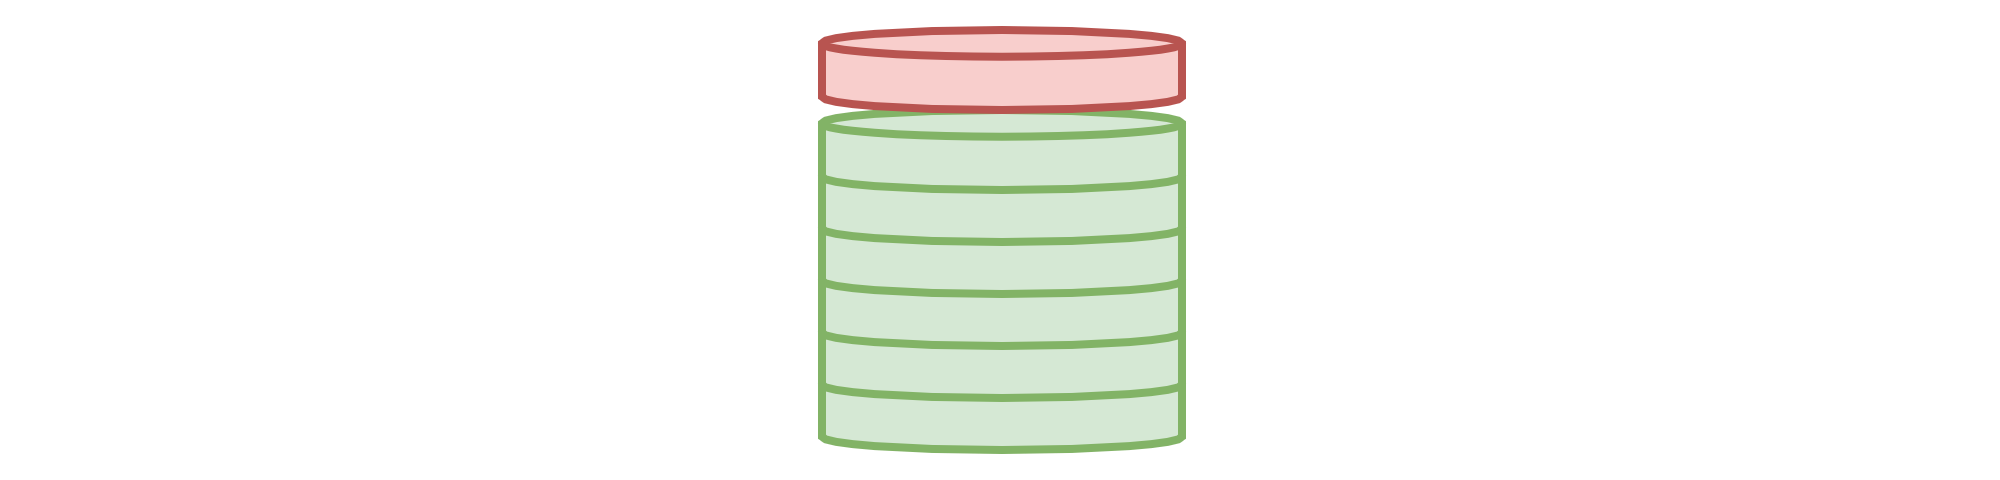
\includegraphics{img-pile.png}\tabularnewline
\emph{Dernier entré, premier sorti} (en anglais \textbf{LIFO} pour
\emph{last in, first out})\tabularnewline
\bottomrule
\end{longtable}

    Dans une \textbf{file} (en anglais \emph{queue}), chaque opération
\texttt{defile} retire l'élément \emph{qui avait été ajouté} le premier.
Pour imaginer cette structure, on pense à une file d'attente dans
laquelle (1) les personnes arrivent à tour de rôle, (2) patientent et
(3) sont servies dans leur ordre d'arrivé.

\begin{longtable}[]{@{}c@{}}
\toprule
\endhead
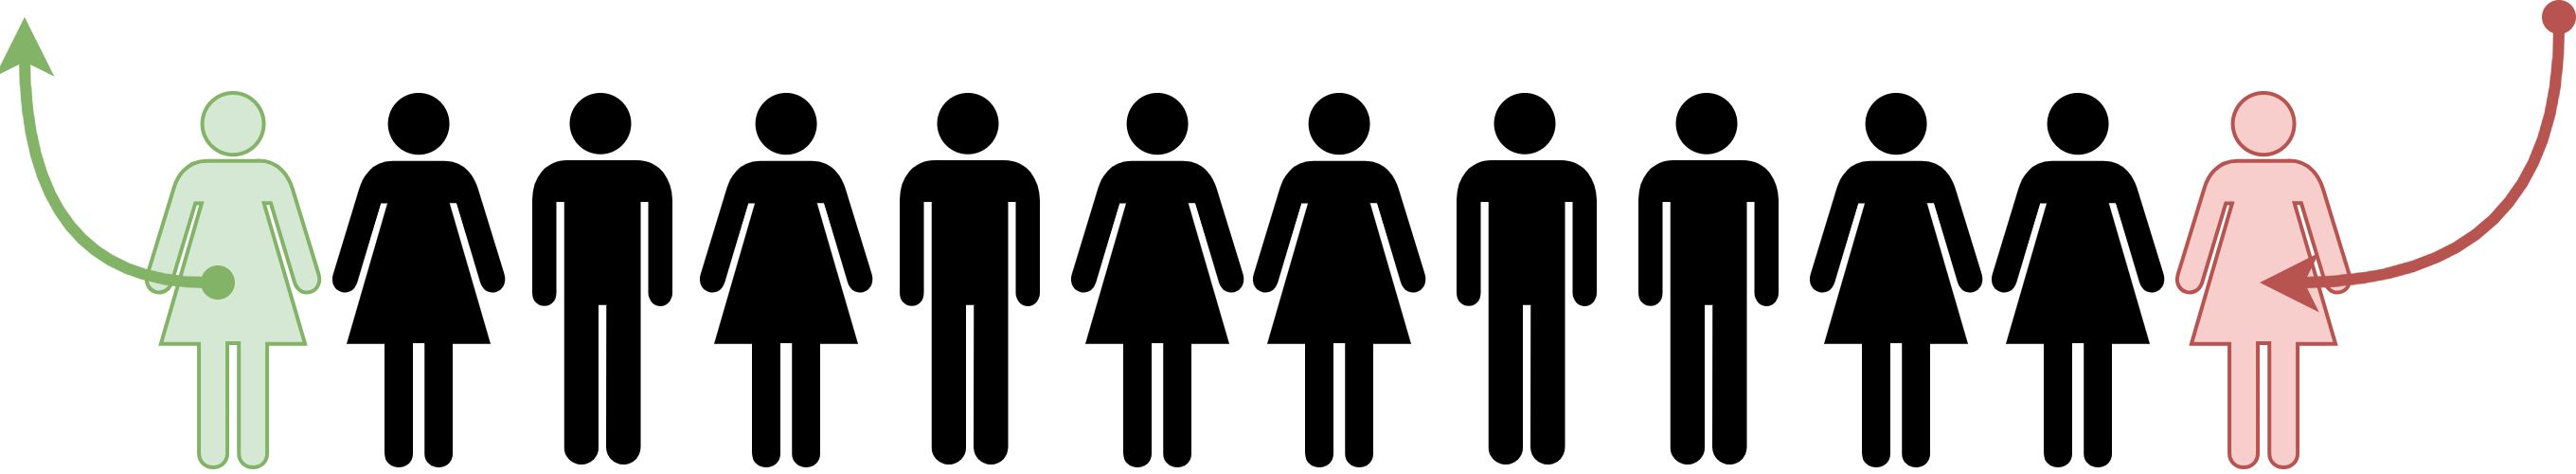
\includegraphics{img-file.png}\tabularnewline
\emph{Premier arrivé, premier sorti} (en anglais \textbf{FIFO} pour
\emph{first in, first out})\tabularnewline
\bottomrule
\end{longtable}

    \hypertarget{interface-commune-aux-piles-et-aux-files}{%
\subsection{6.2 --- Interface commune aux piles et aux
files}\label{interface-commune-aux-piles-et-aux-files}}

    Classiquement, chacune de ces deux structures a une \textbf{interface}
proposant au minimum les quatre opérations suivantes :

\begin{longtable}[]{@{}ccl@{}}
\toprule
\endhead
\textbf{pile} & \textbf{file} & \textbf{opérations}\tabularnewline
\texttt{Pile()} & \texttt{File()} & créer une structure initialement
vide\tabularnewline
\texttt{est\_vide()} & \texttt{est\_vide()} & tester si une structure
est vide\tabularnewline
\texttt{empile()} & \texttt{enfile()} & ajouter un élément à une
structure\tabularnewline
\texttt{depile()} & \texttt{defile()} & retirer et obtenir un élément
d'une structure\tabularnewline
\bottomrule
\end{longtable}

    Comme pour les tableaux et les listes chaînées, on préconisé pour les
piles et les files une \textbf{structures homogènes}. C'est-à-dire que
tous les éléments stockés aient le même type.

    Dans ce cours, nos structures de pile et de file seront considérées
\textbf{mutables} : chaque opération d'ajout ou de retrait d'un élément
\textbf{modifie la pile ou la file} à laquelle elle s'applique.

Mais il aurait été tout à fait possible d'en décider autrement.

    \hypertarget{interface-et-utilisation-dune-pile}{%
\subsection{6.3 --- Interface et utilisation d'une
pile}\label{interface-et-utilisation-dune-pile}}

    Détaillons l'interface des piles.

\begin{longtable}[]{@{}ll@{}}
\toprule
\begin{minipage}[b]{0.47\columnwidth}\raggedright
interface\strut
\end{minipage} & \begin{minipage}[b]{0.47\columnwidth}\raggedright
explications et commentaires\strut
\end{minipage}\tabularnewline
\midrule
\endhead
\begin{minipage}[t]{0.47\columnwidth}\raggedright
\texttt{Pile{[}T{]}}\strut
\end{minipage} & \begin{minipage}[t]{0.47\columnwidth}\raggedright
le type des piles contenant des éléments de type \texttt{T}. Par exemple
\texttt{T} peut être \texttt{int} pour les nombres entiers ou encore
\texttt{str} pour les chaînes de caractères\strut
\end{minipage}\tabularnewline
\begin{minipage}[t]{0.47\columnwidth}\raggedright
\texttt{est\_vide(p:\ Pile{[}T{]})\ -\textgreater{}\ bool}\strut
\end{minipage} & \begin{minipage}[t]{0.47\columnwidth}\raggedright
prend en paramètre une pile \texttt{p} et renvoie un booléen indiquant
si la pile est vide ou pas\strut
\end{minipage}\tabularnewline
\begin{minipage}[t]{0.47\columnwidth}\raggedright
\texttt{creer\_pile()\ -\textgreater{}\ Pile{[}T{]}}\strut
\end{minipage} & \begin{minipage}[t]{0.47\columnwidth}\raggedright
aucun paramètre et renvoie une pile vide capable de contenir n'importe
quel type d'élément \texttt{T}\strut
\end{minipage}\tabularnewline
\begin{minipage}[t]{0.47\columnwidth}\raggedright
\texttt{empiler(p:\ Pile{[}T{]},\ e:\ T)\ -\textgreater{}\ None}\strut
\end{minipage} & \begin{minipage}[t]{0.47\columnwidth}\raggedright
ajout de l'élément \texttt{e} au sommet de la pile \texttt{p}
(\emph{push} en anglais), fonction qui prend en paramètre une pile
\texttt{p} et l'élément \texttt{e} de type \texttt{T} homogène avec
celui des éléments de la pile\strut
\end{minipage}\tabularnewline
\begin{minipage}[t]{0.47\columnwidth}\raggedright
\texttt{depiler(p:\ Pile{[}T{]})\ -\textgreater{}\ T}\strut
\end{minipage} & \begin{minipage}[t]{0.47\columnwidth}\raggedright
retrait de l'élément au sommet de la pile \texttt{p} (\emph{pop} en
anglais) qui prend en paramètre la pile \texttt{p} et renvoie l'élément
qui en a été retiré. On suppose que la pile est non vide et une
exception est levée le cas échéant\strut
\end{minipage}\tabularnewline
\bottomrule
\end{longtable}

    Exemple d'utilisation des piles : Considérons un navigateur web dans
lequel on s'intéresse à deux opérations : \textbf{aller} à une nouvelle
page et \textbf{revenir} à la page précédente. On veut que le bouton de
retour en arrière permette de remonter une à une les pages précédentes,
et ce jusqu'au début de la navigation.

En plus de l'adresse courante, qui peut être stockée dans une variable à
part, il nous faut donc conserver l'ensemble des pages précédentes
auxquelles il est possible de revenir. \emph{Puisque le retour en
arrière se fait vers la dernière page qui a été quittée}, la discipline
\textbf{\emph{dernier entré, premier sorti}} des piles est exactement ce
dont nous avons besoin pour cet ensemble.

    \hypertarget{interface-et-utilisation-dune-file}{%
\subsection{6.4 --- Interface et utilisation d'une
file}\label{interface-et-utilisation-dune-file}}

    Comme pour les piles, on note \texttt{File{[}T{]}} le type des files
contenant des éléments de type \texttt{T}.

\begin{longtable}[]{@{}ll@{}}
\toprule
\begin{minipage}[b]{0.47\columnwidth}\raggedright
\textbf{interface}\strut
\end{minipage} & \begin{minipage}[b]{0.47\columnwidth}\raggedright
\textbf{explications et commentaires}\strut
\end{minipage}\tabularnewline
\midrule
\endhead
\begin{minipage}[t]{0.47\columnwidth}\raggedright
\texttt{File{[}T{]}}\strut
\end{minipage} & \begin{minipage}[t]{0.47\columnwidth}\raggedright
le type des files contenant des éléments de type \texttt{T}\strut
\end{minipage}\tabularnewline
\begin{minipage}[t]{0.47\columnwidth}\raggedright
\texttt{creer\_file()\ -\textgreater{}\ File{[}T{]}}\strut
\end{minipage} & \begin{minipage}[t]{0.47\columnwidth}\raggedright
créer une file vide\strut
\end{minipage}\tabularnewline
\begin{minipage}[t]{0.47\columnwidth}\raggedright
\texttt{est\_vide(f:\ File{[}T{]})\ -\textgreater{}\ bool}\strut
\end{minipage} & \begin{minipage}[t]{0.47\columnwidth}\raggedright
renvoie \texttt{True} si \texttt{f} est vide et \texttt{False}
sinon\strut
\end{minipage}\tabularnewline
\begin{minipage}[t]{0.47\columnwidth}\raggedright
\texttt{enfiler(f:\ File{[}T{]},\ e)\ -\textgreater{}\ None}\strut
\end{minipage} & \begin{minipage}[t]{0.47\columnwidth}\raggedright
ajoute l'élément \texttt{e} à la fin de la file \texttt{f}\strut
\end{minipage}\tabularnewline
\begin{minipage}[t]{0.47\columnwidth}\raggedright
\texttt{defiler(f:\ File{[}T{]})\ -\textgreater{}\ T}\strut
\end{minipage} & \begin{minipage}[t]{0.47\columnwidth}\raggedright
retirer et renvoyer l'élément situé au début de la file \texttt{f}\strut
\end{minipage}\tabularnewline
\bottomrule
\end{longtable}

    Exemple d'utilisation des files : Considérons le jeu de cartes de la
bataille. Chaque joueur possède un paquet de cartes et pose à chaque
manche la carte prise \textbf{sur le dessus du paquet}. Le vainqueur de
la manche récupère alors les cartes posées, pour les placer
\textbf{au-dessous de son paquet}.

En plus des cartes posées au centre de la table nous avons besoin de
conserver en mémoire le paquet de cartes de chaque joueur. \emph{Puisque
les cartes sont remises dans un paquet à une extrémité et prélevées à
l'autre}, la discipline \textbf{\emph{premier entré, premier sorti}} des
files est exactement ce dont nous avons besoin pour chacun de ces
ensembles.

    \hypertarget{ruxe9alisation-dune-pile-avec-une-liste-chauxeenuxe9e}{%
\subsection{6.5 --- Réalisation d'une pile avec une liste
chaînée}\label{ruxe9alisation-dune-pile-avec-une-liste-chauxeenuxe9e}}

    La structure de \textbf{liste chaînée} donne une manière élémentaire de
réaliser une pile. Empiler un nouvel élément revient à ajouter un
nouveau maillon en tête de liste, tandis que dépiler un élément revient
à supprimer le maillon de tête.

On peut ainsi construire une classe \texttt{Pile} définie par un unique
attribut contenu associé à l'ensemble des éléments de la pile, stockés
sous la forme d'une liste chaînée.

    Implémenter le constructeur de la classe \texttt{Pile} qui construit une
pile vide en définissant son attribut \texttt{contenu} comme la liste
vide \texttt{None}.

Exemple et test :

\begin{verbatim}
    >>> p = Pile()
    >>> print(p.contenu)
    None
\end{verbatim}

        {\scriptsize
    \begin{tcolorbox}[breakable, size=fbox, boxrule=1pt, pad at break*=1mm,colback=cellbackground, colframe=cellborder]
\prompt{In}{incolor}{ }{\boxspacing}
\begin{Verbatim}[commandchars=\\\{\}]
\PY{k+kn}{from} \PY{n+nn}{doctest} \PY{k+kn}{import} \PY{n}{testmod}


\PY{k}{class} \PY{n+nc}{Maillon}\PY{p}{:}
    \PY{l+s+sd}{\PYZdq{}\PYZdq{}\PYZdq{} Maillon d\PYZsq{}une liste chaînée \PYZdq{}\PYZdq{}\PYZdq{}}
    \PY{k}{def} \PY{n+nf+fm}{\PYZus{}\PYZus{}init\PYZus{}\PYZus{}}\PY{p}{(}\PY{n+nb+bp}{self}\PY{p}{,} \PY{n}{valeur}\PY{p}{,} \PY{n}{suivant}\PY{p}{)}\PY{p}{:}
        \PY{n+nb+bp}{self}\PY{o}{.}\PY{n}{valeur}  \PY{o}{=} \PY{n}{valeur}
        \PY{n+nb+bp}{self}\PY{o}{.}\PY{n}{suivant} \PY{o}{=} \PY{n}{suivant}

\PY{k}{class} \PY{n+nc}{Pile}\PY{p}{:}
    \PY{l+s+sd}{\PYZdq{}\PYZdq{}\PYZdq{}}
\PY{l+s+sd}{    Encapsulation des piles à l\PYZsq{}aide des Maillons de listes chaînées.}
\PY{l+s+sd}{    \PYZdq{}\PYZdq{}\PYZdq{}}
    \PY{k}{def} \PY{n+nf+fm}{\PYZus{}\PYZus{}init\PYZus{}\PYZus{}}\PY{p}{(}\PY{n+nb+bp}{self}\PY{p}{)}\PY{p}{:}
        \PY{l+s+sd}{\PYZdq{}\PYZdq{}\PYZdq{}}
\PY{l+s+sd}{        Constructeur de Pile.}

\PY{l+s+sd}{        Exemple et tests:}
\PY{l+s+sd}{        \PYZgt{}\PYZgt{}\PYZgt{} p = Pile()}
\PY{l+s+sd}{        \PYZgt{}\PYZgt{}\PYZgt{} print(p.contenu)}
\PY{l+s+sd}{        None}
\PY{l+s+sd}{        \PYZdq{}\PYZdq{}\PYZdq{}}
        \PY{n+nb+bp}{self}\PY{o}{.}\PY{n}{contenu} \PY{o}{=} \PY{k+kc}{None}


\PY{c+c1}{\PYZsh{} tests de la classe}
\PY{n}{testmod}\PY{p}{(}\PY{p}{)}
\end{Verbatim}
\end{tcolorbox}
    }

    Étendre la classe \texttt{Pile} en implémentant la méthode
\texttt{est\_vide}.

Exemples et tests :

\begin{verbatim}
    >>> p = Pile()
    >>> print(p.est_vide())
    True
    >>> p.contenu = Maillon(1, None)
    >>> print(p.est_vide())
    False
\end{verbatim}

        {\scriptsize
    \begin{tcolorbox}[breakable, size=fbox, boxrule=1pt, pad at break*=1mm,colback=cellbackground, colframe=cellborder]
\prompt{In}{incolor}{ }{\boxspacing}
\begin{Verbatim}[commandchars=\\\{\}]
\PY{c+c1}{\PYZsh{} attention, lorsqu\PYZsq{}on implémente une }
\PY{c+c1}{\PYZsh{} classe en une seule fois, il faut écrire}
\PY{c+c1}{\PYZsh{} `class Pile:`.}
\PY{c+c1}{\PYZsh{} La syntaxe `class Pile(Ma\PYZus{}Classe):` est utilisée}
\PY{c+c1}{\PYZsh{} dans ce notebook (et dans les juges en lignes)}
\PY{c+c1}{\PYZsh{} pour étendre la classe existante Ma\PYZus{}Classe et lui}
\PY{c+c1}{\PYZsh{} ajouter de nouvelles méthodes.}
\PY{c+c1}{\PYZsh{}}
\PY{c+c1}{\PYZsh{} Ici, la classe Pile s\PYZsq{}étend elle même !}

\PY{k}{class} \PY{n+nc}{Pile}\PY{p}{(}\PY{n}{Pile}\PY{p}{)}\PY{p}{:}
    \PY{k}{def} \PY{n+nf}{est\PYZus{}vide}\PY{p}{(}\PY{n+nb+bp}{self}\PY{p}{)} \PY{o}{\PYZhy{}}\PY{o}{\PYZgt{}} \PY{n+nb}{bool}\PY{p}{:}
        \PY{l+s+sd}{\PYZdq{}\PYZdq{}\PYZdq{}}
\PY{l+s+sd}{        Est ce que la pile est vide ?}

\PY{l+s+sd}{        Returns:}
\PY{l+s+sd}{            bool: True si et seulement si la pile est vide}

\PY{l+s+sd}{        Exemple et test:}
\PY{l+s+sd}{        \PYZgt{}\PYZgt{}\PYZgt{} p = Pile()}
\PY{l+s+sd}{        \PYZgt{}\PYZgt{}\PYZgt{} print(p.est\PYZus{}vide())}
\PY{l+s+sd}{        True}
\PY{l+s+sd}{        \PYZgt{}\PYZgt{}\PYZgt{} p.contenu = Maillon(1, None)}
\PY{l+s+sd}{        \PYZgt{}\PYZgt{}\PYZgt{} print(p.est\PYZus{}vide())}
\PY{l+s+sd}{        False}
\PY{l+s+sd}{        \PYZdq{}\PYZdq{}\PYZdq{}}
        \PY{k}{return} \PY{n+nb+bp}{self}\PY{o}{.}\PY{n}{contenu} \PY{o+ow}{is} \PY{k+kc}{None}


\PY{n}{testmod}\PY{p}{(}\PY{p}{)}
\end{Verbatim}
\end{tcolorbox}
    }

    Implémenter la méthode \texttt{empile} dans la classe \texttt{Pile}.
Pour cela construire une nouvelle liste chaînée dont le premier maillon
contient :

\begin{itemize}
\tightlist
\item
  valeur : la valeur à empiler
\item
  suivant : le premier maillon de la liste d'origine de la pile
\end{itemize}

Puis mettre à jour le contenu de la pile avec cette nouvelle liste.

Exemple et tests:

\begin{verbatim}
    >>> p = Pile()
    >>> p.empiler(1)
    >>> assert not p.est_vide()
    >>> print(p.contenu.valeur)
    1
    >>> p.empiler(2)
    >>> print(p.contenu.valeur)
    2
\end{verbatim}

        {\scriptsize
    \begin{tcolorbox}[breakable, size=fbox, boxrule=1pt, pad at break*=1mm,colback=cellbackground, colframe=cellborder]
\prompt{In}{incolor}{ }{\boxspacing}
\begin{Verbatim}[commandchars=\\\{\}]
\PY{c+c1}{\PYZsh{} attention, lorsqu\PYZsq{}on implémente une }
\PY{c+c1}{\PYZsh{} classe en une seule fois, il faut écrire}
\PY{c+c1}{\PYZsh{} `class Pile:`.}
\PY{c+c1}{\PYZsh{} La syntaxe `class Pile(Ma\PYZus{}Classe):` est utilisée}
\PY{c+c1}{\PYZsh{} dans ce notebook (et dans les juges en lignes)}
\PY{c+c1}{\PYZsh{} pour étendre la classe existante Ma\PYZus{}Classe et lui}
\PY{c+c1}{\PYZsh{} ajouter de nouvelles méthodes.}
\PY{c+c1}{\PYZsh{}}
\PY{c+c1}{\PYZsh{} Ici, la classe Pile s\PYZsq{}étend elle même !}

\PY{k}{class} \PY{n+nc}{Pile}\PY{p}{(}\PY{n}{Pile}\PY{p}{)}\PY{p}{:}
    \PY{k}{def} \PY{n+nf}{empiler}\PY{p}{(}\PY{n+nb+bp}{self}\PY{p}{,} \PY{n}{valeur}\PY{p}{)}\PY{p}{:}
            \PY{l+s+sd}{\PYZdq{}\PYZdq{}\PYZdq{}}
\PY{l+s+sd}{            Empile valeur dans la pile courante.}

\PY{l+s+sd}{            Args:}
\PY{l+s+sd}{                valeur (T): valeur à empiler}

\PY{l+s+sd}{            Exemple et tests:}
\PY{l+s+sd}{            \PYZgt{}\PYZgt{}\PYZgt{} p = Pile()}
\PY{l+s+sd}{            \PYZgt{}\PYZgt{}\PYZgt{} p.empiler(1)}
\PY{l+s+sd}{            \PYZgt{}\PYZgt{}\PYZgt{} assert not p.est\PYZus{}vide()}
\PY{l+s+sd}{            \PYZgt{}\PYZgt{}\PYZgt{} print(p.contenu.valeur)}
\PY{l+s+sd}{            1}
\PY{l+s+sd}{            \PYZgt{}\PYZgt{}\PYZgt{} p.empiler(2)}
\PY{l+s+sd}{            \PYZgt{}\PYZgt{}\PYZgt{} print(p.contenu.valeur)}
\PY{l+s+sd}{            2}
\PY{l+s+sd}{            \PYZdq{}\PYZdq{}\PYZdq{}}
            \PY{n}{tete\PYZus{}courante} \PY{o}{=} \PY{n+nb+bp}{self}\PY{o}{.}\PY{n}{contenu}
            \PY{n}{tete\PYZus{}nouvelle} \PY{o}{=} \PY{n}{Maillon}\PY{p}{(}\PY{n}{valeur}\PY{p}{,} \PY{n}{tete\PYZus{}courante}\PY{p}{)}
            \PY{n+nb+bp}{self}\PY{o}{.}\PY{n}{contenu} \PY{o}{=} \PY{n}{tete\PYZus{}nouvelle}

            \PY{c+c1}{\PYZsh{} version courte ;)}
            \PY{c+c1}{\PYZsh{} self.contenu = Maillon(valeur, self.contenu)}


\PY{n}{testmod}\PY{p}{(}\PY{p}{)}
\end{Verbatim}
\end{tcolorbox}
    }

    Pour finir, implémenter \texttt{depiler} afin de récupérer la valeur au
sommet de la pile.

Si la pile est vide, lever une exception indiquant :
\texttt{"IndexError:\ depiler\ sur\ une\ pile\ vide"}.

Sinon, il faut récupérer la valeur du premier maillon puis retirer ce
maillon de la liste chaînée. Pour cela, le nouveau maillon de tête doit
être le maillon suivant du maillon supprimé.

Enfin, après la mise à jour de la liste chaînée, il faut renvoyer la
valeur qui avait été prélevée dans le maillon de tête d'origine.

Exemple et tests:

\begin{verbatim}
    >>> p = Pile()
    >>> p.empiler(1)
    >>> p.empiler(2)
    >>> v = p.depiler()
    >>> print(v)
    2
    >>> v = p.depiler()
    >>> print(v)
    1
    >>> v = p.depiler()
    Traceback (most recent call last):
    IndexError: depiler sur une pile vide
\end{verbatim}

        {\scriptsize
    \begin{tcolorbox}[breakable, size=fbox, boxrule=1pt, pad at break*=1mm,colback=cellbackground, colframe=cellborder]
\prompt{In}{incolor}{ }{\boxspacing}
\begin{Verbatim}[commandchars=\\\{\}]
\PY{c+c1}{\PYZsh{} attention, lorsqu\PYZsq{}on implémente une }
\PY{c+c1}{\PYZsh{} classe en une seule fois, il faut écrire}
\PY{c+c1}{\PYZsh{} `class Pile:`.}
\PY{c+c1}{\PYZsh{} La syntaxe `class Pile(Ma\PYZus{}Classe):` est utilisée}
\PY{c+c1}{\PYZsh{} dans ce notebook (et dans les juges en lignes)}
\PY{c+c1}{\PYZsh{} pour étendre la classe existante Ma\PYZus{}Classe et lui}
\PY{c+c1}{\PYZsh{} ajouter de nouvelles méthodes.}
\PY{c+c1}{\PYZsh{}}
\PY{c+c1}{\PYZsh{} Ici, la classe Pile s\PYZsq{}étend elle même !}


\PY{k}{class} \PY{n+nc}{Pile}\PY{p}{(}\PY{n}{Pile}\PY{p}{)}\PY{p}{:}
    \PY{k}{def} \PY{n+nf}{depiler}\PY{p}{(}\PY{n+nb+bp}{self}\PY{p}{)}\PY{p}{:}
        \PY{l+s+sd}{\PYZdq{}\PYZdq{}\PYZdq{}}
\PY{l+s+sd}{        Dépile la valeur de tête de la pile.}

\PY{l+s+sd}{        Raises:}
\PY{l+s+sd}{            IndexError: si la pile est vide}

\PY{l+s+sd}{        Returns:}
\PY{l+s+sd}{            T: valeur de tête de la pile}

\PY{l+s+sd}{        Exemple et tests:}
\PY{l+s+sd}{        \PYZgt{}\PYZgt{}\PYZgt{} p = Pile()}
\PY{l+s+sd}{        \PYZgt{}\PYZgt{}\PYZgt{} p.empiler(1)}
\PY{l+s+sd}{        \PYZgt{}\PYZgt{}\PYZgt{} p.empiler(2)}
\PY{l+s+sd}{        \PYZgt{}\PYZgt{}\PYZgt{} v = p.depiler()}
\PY{l+s+sd}{        \PYZgt{}\PYZgt{}\PYZgt{} print(v)}
\PY{l+s+sd}{        2}
\PY{l+s+sd}{        \PYZgt{}\PYZgt{}\PYZgt{} v = p.depiler()}
\PY{l+s+sd}{        \PYZgt{}\PYZgt{}\PYZgt{} print(v)}
\PY{l+s+sd}{        1}
\PY{l+s+sd}{        \PYZgt{}\PYZgt{}\PYZgt{} v = p.depiler()}
\PY{l+s+sd}{        Traceback (most recent call last):}
\PY{l+s+sd}{        IndexError: depiler sur une pile vide}
\PY{l+s+sd}{        \PYZdq{}\PYZdq{}\PYZdq{}}
        \PY{k}{if} \PY{n+nb+bp}{self}\PY{o}{.}\PY{n}{est\PYZus{}vide}\PY{p}{(}\PY{p}{)}\PY{p}{:}
            \PY{k}{raise} \PY{n+ne}{IndexError}\PY{p}{(}\PY{l+s+s2}{\PYZdq{}}\PY{l+s+s2}{depiler sur une pile vide}\PY{l+s+s2}{\PYZdq{}}\PY{p}{)}
        
        \PY{n}{tete} \PY{o}{=} \PY{n+nb+bp}{self}\PY{o}{.}\PY{n}{contenu}
        \PY{n}{valeur\PYZus{}tete} \PY{o}{=} \PY{n}{tete}\PY{o}{.}\PY{n}{valeur}
        \PY{n}{maillon\PYZus{}suivant} \PY{o}{=} \PY{n}{tete}\PY{o}{.}\PY{n}{suivant}
        \PY{n+nb+bp}{self}\PY{o}{.}\PY{n}{contenu} \PY{o}{=} \PY{n}{maillon\PYZus{}suivant}
        
        \PY{k}{return} \PY{n}{valeur\PYZus{}tete}


\PY{n}{testmod}\PY{p}{(}\PY{p}{)}
\end{Verbatim}
\end{tcolorbox}
    }

    \hypertarget{ruxe9alisation-dune-file-avec-une-liste-mutable}{%
\subsection{6.6 --- Réalisation d'une file avec une liste
mutable}\label{ruxe9alisation-dune-file-avec-une-liste-mutable}}

    La structure de liste chaînée donne également une manière de réaliser
une file, à condition de considérer la variante des \emph{listes
chaînées mutables}.

En effet, on peut retirer l'élément de tête en retirant le maillon de
tête. MAIS, l'ajout d'un nouvel élément à l'arrière de la file revient à
ajouter un nouveau maillon en queue de liste. \textbf{Une mutation
intervient} à cet endroit : alors que le maillon qui était le dernier de
la liste chaînée avant l'ajout n'avait pas de suivant définie, il a
comme suivant après l'ajout le nouveau maillon créé pour le nouvel
élément.

    Autre différence avec la structure de pile, il faut accéder
\emph{efficacement} au dernier maillon.

Pour cela, le plus intéressant est de conserver dans notre structure de
donnée un attribut permettant d'accéder directement au dernier maillon.

    On peut ainsi construire une classe \texttt{File} dont le constructeur
définit deux attributs, l'un appelé \texttt{tete} et l'autre appelé
\texttt{queue}, et désignant respectivement le premier maillon et le
dernier maillon de la liste chaînée utilisée pour stocker les éléments.

Implémenter le constructeur de la classe \texttt{File} qui définit les
deux attributs \texttt{tete} et \texttt{queue} et les initialise à
\texttt{None}.

Exemples et tests:

\begin{verbatim}
    >>> f = File()
    >>> print(f.tete)
    None
    >>> print(f.queue)
    None
\end{verbatim}

        {\scriptsize
    \begin{tcolorbox}[breakable, size=fbox, boxrule=1pt, pad at break*=1mm,colback=cellbackground, colframe=cellborder]
\prompt{In}{incolor}{4}{\boxspacing}
\begin{Verbatim}[commandchars=\\\{\}]
\PY{k}{class} \PY{n+nc}{Maillon}\PY{p}{:}
    \PY{l+s+sd}{\PYZdq{}\PYZdq{}\PYZdq{} Maillon d\PYZsq{}une liste chaînée \PYZdq{}\PYZdq{}\PYZdq{}}
    \PY{k}{def} \PY{n+nf+fm}{\PYZus{}\PYZus{}init\PYZus{}\PYZus{}}\PY{p}{(}\PY{n+nb+bp}{self}\PY{p}{,} \PY{n}{valeur}\PY{p}{,} \PY{n}{suivant}\PY{p}{)}\PY{p}{:}
        \PY{n+nb+bp}{self}\PY{o}{.}\PY{n}{valeur}  \PY{o}{=} \PY{n}{valeur}
        \PY{n+nb+bp}{self}\PY{o}{.}\PY{n}{suivant} \PY{o}{=} \PY{n}{suivant}

\PY{k}{class} \PY{n+nc}{File}\PY{p}{:}
    \PY{k}{def} \PY{n+nf+fm}{\PYZus{}\PYZus{}init\PYZus{}\PYZus{}}\PY{p}{(}\PY{n+nb+bp}{self}\PY{p}{)}\PY{p}{:}
        \PY{l+s+sd}{\PYZdq{}\PYZdq{}\PYZdq{}}
\PY{l+s+sd}{        Exemples et tests:}
\PY{l+s+sd}{        \PYZgt{}\PYZgt{}\PYZgt{} f = File()}
\PY{l+s+sd}{        \PYZgt{}\PYZgt{}\PYZgt{} print(f.tete)}
\PY{l+s+sd}{        None}
\PY{l+s+sd}{        \PYZgt{}\PYZgt{}\PYZgt{} print(f.queue)}
\PY{l+s+sd}{        None}
\PY{l+s+sd}{        \PYZdq{}\PYZdq{}\PYZdq{}}
        \PY{n+nb+bp}{self}\PY{o}{.}\PY{n}{tete}  \PY{o}{=} \PY{k+kc}{None}
        \PY{n+nb+bp}{self}\PY{o}{.}\PY{n}{queue} \PY{o}{=} \PY{k+kc}{None}


\PY{n}{testmod}\PY{p}{(}\PY{p}{)}
\end{Verbatim}
\end{tcolorbox}
    }

            \begin{tcolorbox}[breakable, size=fbox, boxrule=.5pt, pad at break*=1mm, opacityfill=0]
\prompt{Out}{outcolor}{4}{\boxspacing}
\begin{Verbatim}[commandchars=\\\{\}]
TestResults(failed=0, attempted=3)
\end{Verbatim}
\end{tcolorbox}
        
    La file vide est caractérisée par le fait qu'elle ne contient aucun
maillon. En conséquence, sa tête et sa queue sont indéfinies. En outre,
l'un comme l'autre ne peut valoir \texttt{None} que dans ce cas. Pour
tester la vacuité de la file, il suffit donc de consulter l'un des deux
attributs.

Implémenter la méthode \texttt{est\_vide()} qui renvoie \texttt{True} si
et seulement si l'attribut \texttt{tete} vaut \texttt{None}.

Exemples et tests:

\begin{verbatim}
    >>> f = File()
    >>> print(f.est_vide())
    True
    >>> f.tete = Maillon(1, None)
    >>> print(f.est_vide())
    False
\end{verbatim}

        {\scriptsize
    \begin{tcolorbox}[breakable, size=fbox, boxrule=1pt, pad at break*=1mm,colback=cellbackground, colframe=cellborder]
\prompt{In}{incolor}{5}{\boxspacing}
\begin{Verbatim}[commandchars=\\\{\}]
\PY{c+c1}{\PYZsh{} attention, lorsqu\PYZsq{}on implémente une }
\PY{c+c1}{\PYZsh{} classe en une seule fois, il faut écrire}
\PY{c+c1}{\PYZsh{} `class File:`.}
\PY{c+c1}{\PYZsh{} La syntaxe `class File(Ma\PYZus{}Classe):` est utilisée}
\PY{c+c1}{\PYZsh{} dans ce notebook (et dans les juges en lignes)}
\PY{c+c1}{\PYZsh{} pour étendre la classe existante Ma\PYZus{}Classe et lui}
\PY{c+c1}{\PYZsh{} ajouter de nouvelles méthodes.}
\PY{c+c1}{\PYZsh{}}
\PY{c+c1}{\PYZsh{} Ici, la classe File s\PYZsq{}étend elle même !}
 
\PY{k}{class} \PY{n+nc}{File}\PY{p}{(}\PY{n}{File}\PY{p}{)}\PY{p}{:}

    \PY{k}{def} \PY{n+nf}{est\PYZus{}vide}\PY{p}{(}\PY{n+nb+bp}{self}\PY{p}{)}\PY{p}{:}
        \PY{l+s+sd}{\PYZdq{}\PYZdq{}\PYZdq{}}
\PY{l+s+sd}{        Est ce que la file est vide?}

\PY{l+s+sd}{        Returns:}
\PY{l+s+sd}{            bool: True ssi la file est vide}
\PY{l+s+sd}{        }
\PY{l+s+sd}{        Exemples et tests:}
\PY{l+s+sd}{        \PYZgt{}\PYZgt{}\PYZgt{} f = File()}
\PY{l+s+sd}{        \PYZgt{}\PYZgt{}\PYZgt{} print(f.est\PYZus{}vide())}
\PY{l+s+sd}{        True}
\PY{l+s+sd}{        \PYZgt{}\PYZgt{}\PYZgt{} f.tete = Maillon(1, None)}
\PY{l+s+sd}{        \PYZgt{}\PYZgt{}\PYZgt{} print(f.est\PYZus{}vide())}
\PY{l+s+sd}{        False}
\PY{l+s+sd}{        \PYZdq{}\PYZdq{}\PYZdq{}}
        \PY{k}{return} \PY{n+nb+bp}{self}\PY{o}{.}\PY{n}{tete} \PY{o+ow}{is} \PY{k+kc}{None}
    


\PY{n}{testmod}\PY{p}{(}\PY{p}{)}
\end{Verbatim}
\end{tcolorbox}
    }

            \begin{tcolorbox}[breakable, size=fbox, boxrule=.5pt, pad at break*=1mm, opacityfill=0]
\prompt{Out}{outcolor}{5}{\boxspacing}
\begin{Verbatim}[commandchars=\\\{\}]
TestResults(failed=0, attempted=4)
\end{Verbatim}
\end{tcolorbox}
        
    L'ajout d'un nouvel élément à l'arrière de la file demande de créer un
nouveau maillon. Ce maillon prend la dernière place, et n'a donc pas de
maillon suivant.

Ce maillon est alors définie comme suivant le maillon de queue actuel.

On a cependant besoin de traiter le cas particulier où il n'existe pas
de maillon de queue, qui correspond à une file initialement vide. Dans
ce cas le nouveau maillon devient l'unique maillon de la file, et donc
son maillon de tête.

Pour finir, dans tous les cas, notre nouveau maillon devient en outre le
nouveau maillon de de queue de la file.

    En suivant l'algorithme décrit ci-dessus, implémenter la méthode
\texttt{enfiler} qui admet comme argument une \texttt{valeur} à ajouter
en queue de file.

Exemples et tests:

\begin{verbatim}
    >>> f = File()
    >>> f.enfiler(1)
    >>> print(f.tete.valeur)
    1
    >>> print(f.queue.valeur)
    1
    >>> f.enfiler(2)
    >>> f.enfiler(3)
    >>> print(f.tete.valeur)
    1
    >>> print(f.queue.valeur)
    3
\end{verbatim}

        {\scriptsize
    \begin{tcolorbox}[breakable, size=fbox, boxrule=1pt, pad at break*=1mm,colback=cellbackground, colframe=cellborder]
\prompt{In}{incolor}{6}{\boxspacing}
\begin{Verbatim}[commandchars=\\\{\}]
\PY{k}{class} \PY{n+nc}{File}\PY{p}{(}\PY{n}{File}\PY{p}{)}\PY{p}{:}
    \PY{k}{def} \PY{n+nf}{enfiler}\PY{p}{(}\PY{n+nb+bp}{self}\PY{p}{,} \PY{n}{valeur}\PY{p}{)}\PY{p}{:}
        \PY{l+s+sd}{\PYZdq{}\PYZdq{}\PYZdq{}}
\PY{l+s+sd}{        Ajoute la valeur à la fin de la file}

\PY{l+s+sd}{        Args:}
\PY{l+s+sd}{            valeur (T): valeur à ajouter}
\PY{l+s+sd}{        }
\PY{l+s+sd}{        Exemples et tests:}
\PY{l+s+sd}{        \PYZgt{}\PYZgt{}\PYZgt{} f = File()}
\PY{l+s+sd}{        \PYZgt{}\PYZgt{}\PYZgt{} f.enfiler(1)}
\PY{l+s+sd}{        \PYZgt{}\PYZgt{}\PYZgt{} print(f.tete.valeur)}
\PY{l+s+sd}{        1}
\PY{l+s+sd}{        \PYZgt{}\PYZgt{}\PYZgt{} print(f.queue.valeur)}
\PY{l+s+sd}{        1}
\PY{l+s+sd}{        \PYZgt{}\PYZgt{}\PYZgt{} f.enfiler(2)}
\PY{l+s+sd}{        \PYZgt{}\PYZgt{}\PYZgt{} f.enfiler(3)}
\PY{l+s+sd}{        \PYZgt{}\PYZgt{}\PYZgt{} print(f.tete.valeur)}
\PY{l+s+sd}{        1}
\PY{l+s+sd}{        \PYZgt{}\PYZgt{}\PYZgt{} print(f.queue.valeur)}
\PY{l+s+sd}{        3}
\PY{l+s+sd}{        \PYZdq{}\PYZdq{}\PYZdq{}}
        \PY{n}{nouveau} \PY{o}{=} \PY{n}{Maillon}\PY{p}{(}\PY{n}{valeur}\PY{p}{,} \PY{k+kc}{None}\PY{p}{)}

        \PY{k}{if} \PY{n+nb+bp}{self}\PY{o}{.}\PY{n}{est\PYZus{}vide}\PY{p}{(}\PY{p}{)}\PY{p}{:}
            \PY{n+nb+bp}{self}\PY{o}{.}\PY{n}{tete} \PY{o}{=} \PY{n}{nouveau}
        \PY{k}{else}\PY{p}{:}
            \PY{n+nb+bp}{self}\PY{o}{.}\PY{n}{queue}\PY{o}{.}\PY{n}{suivant} \PY{o}{=} \PY{n}{nouveau}
        
        \PY{n+nb+bp}{self}\PY{o}{.}\PY{n}{queue} \PY{o}{=} \PY{n}{nouveau}


\PY{n}{testmod}\PY{p}{(}\PY{p}{)}
\end{Verbatim}
\end{tcolorbox}
    }

            \begin{tcolorbox}[breakable, size=fbox, boxrule=.5pt, pad at break*=1mm, opacityfill=0]
\prompt{Out}{outcolor}{6}{\boxspacing}
\begin{Verbatim}[commandchars=\\\{\}]
TestResults(failed=0, attempted=8)
\end{Verbatim}
\end{tcolorbox}
        
    Pour retirer un élément il s'agit de supprimer le premier maillon de la
file, exactement comme il avait été fait lors de l'utilisation d'une
liste chaînée pour réaliser une pile. Cependant, si le maillon retiré
est le dernier, on veut également redéfinir l'attribut
\texttt{self.queue} à \texttt{None}, afin de maintenir notre invariant
qu'une file vide a ses deux attributs qui valent \texttt{None}.

    Implémenter la méthode \texttt{defiler} qui retire le premier maillon de
la file et renvoie la valeur de ce maillon.

Exemples et tests:

\begin{verbatim}
    >>> f = File()
    >>> f.enfiler(1)
    >>> f.enfiler(2)
    >>> f.enfiler(3)
    >>> print( f.defiler() )
    1
    >>> assert f.queue.valeur == 3
    >>> print( f.defiler() )
    2
    >>> assert f.queue.valeur == 3
    >>> print( f.defiler() )
    3
    >>> assert f.tete  == None
    >>> assert f.queue == None
    >>> f.defiler()
    Traceback (most recent call last):
    IndexError: defiler sur une file vide
\end{verbatim}

        {\scriptsize
    \begin{tcolorbox}[breakable, size=fbox, boxrule=1pt, pad at break*=1mm,colback=cellbackground, colframe=cellborder]
\prompt{In}{incolor}{8}{\boxspacing}
\begin{Verbatim}[commandchars=\\\{\}]
\PY{k}{class} \PY{n+nc}{File}\PY{p}{(}\PY{n}{File}\PY{p}{)}\PY{p}{:}
    \PY{k}{def} \PY{n+nf}{defiler}\PY{p}{(}\PY{n+nb+bp}{self}\PY{p}{)}\PY{p}{:}
        \PY{l+s+sd}{\PYZdq{}\PYZdq{}\PYZdq{}}
\PY{l+s+sd}{        Supprime et renvoie le premier élément de la file}

\PY{l+s+sd}{        Raises:}
\PY{l+s+sd}{            IndexError: si la file est vide}

\PY{l+s+sd}{        Returns:}
\PY{l+s+sd}{            T: valeur du premier élément de la file}
\PY{l+s+sd}{        }
\PY{l+s+sd}{        Exemples et tests:}
\PY{l+s+sd}{        \PYZgt{}\PYZgt{}\PYZgt{} f = File()}
\PY{l+s+sd}{        \PYZgt{}\PYZgt{}\PYZgt{} f.enfiler(1)}
\PY{l+s+sd}{        \PYZgt{}\PYZgt{}\PYZgt{} f.enfiler(2)}
\PY{l+s+sd}{        \PYZgt{}\PYZgt{}\PYZgt{} f.enfiler(3)}
\PY{l+s+sd}{        \PYZgt{}\PYZgt{}\PYZgt{} print( f.defiler() )}
\PY{l+s+sd}{        1}
\PY{l+s+sd}{        \PYZgt{}\PYZgt{}\PYZgt{} assert f.queue.valeur == 3}
\PY{l+s+sd}{        \PYZgt{}\PYZgt{}\PYZgt{} print( f.defiler() )}
\PY{l+s+sd}{        2}
\PY{l+s+sd}{        \PYZgt{}\PYZgt{}\PYZgt{} assert f.queue.valeur == 3}
\PY{l+s+sd}{        \PYZgt{}\PYZgt{}\PYZgt{} print( f.defiler() )}
\PY{l+s+sd}{        3}
\PY{l+s+sd}{        \PYZgt{}\PYZgt{}\PYZgt{} assert f.tete  == None}
\PY{l+s+sd}{        \PYZgt{}\PYZgt{}\PYZgt{} assert f.queue == None}
\PY{l+s+sd}{        \PYZgt{}\PYZgt{}\PYZgt{} f.defiler()}
\PY{l+s+sd}{        Traceback (most recent call last):}
\PY{l+s+sd}{        IndexError: defiler sur une file vide}
\PY{l+s+sd}{        \PYZdq{}\PYZdq{}\PYZdq{}}
        \PY{k}{if} \PY{n+nb+bp}{self}\PY{o}{.}\PY{n}{est\PYZus{}vide}\PY{p}{(}\PY{p}{)}\PY{p}{:}
            \PY{k}{raise} \PY{n+ne}{IndexError}\PY{p}{(}\PY{l+s+s2}{\PYZdq{}}\PY{l+s+s2}{defiler sur une file vide}\PY{l+s+s2}{\PYZdq{}}\PY{p}{)}
        
        \PY{n}{valeur} \PY{o}{=} \PY{n+nb+bp}{self}\PY{o}{.}\PY{n}{tete}\PY{o}{.}\PY{n}{valeur}
        \PY{n+nb+bp}{self}\PY{o}{.}\PY{n}{tete} \PY{o}{=} \PY{n+nb+bp}{self}\PY{o}{.}\PY{n}{tete}\PY{o}{.}\PY{n}{suivant}

        \PY{k}{if} \PY{n+nb+bp}{self}\PY{o}{.}\PY{n}{tete} \PY{o+ow}{is} \PY{k+kc}{None}\PY{p}{:}
            \PY{n+nb+bp}{self}\PY{o}{.}\PY{n}{queue} \PY{o}{=} \PY{k+kc}{None}

        \PY{k}{return} \PY{n}{valeur}


\PY{n}{testmod}\PY{p}{(}\PY{p}{)}
\end{Verbatim}
\end{tcolorbox}
    }

            \begin{tcolorbox}[breakable, size=fbox, boxrule=.5pt, pad at break*=1mm, opacityfill=0]
\prompt{Out}{outcolor}{8}{\boxspacing}
\begin{Verbatim}[commandchars=\\\{\}]
TestResults(failed=0, attempted=12)
\end{Verbatim}
\end{tcolorbox}
        
    \hypertarget{ruxe9alisation-dune-pile-avec-les-tableaux-de-python}{%
\subsection{6.7 --- Réalisation d'une pile avec les tableaux de
Python}\label{ruxe9alisation-dune-pile-avec-les-tableaux-de-python}}

    Les tableaux de Python réalisent également directement une structure de
pile, avec leurs opérations \texttt{append} et \texttt{pop} qui
s'exécutent en moyenne en temps constant. Cette richesse des tableaux
redimensionnables propre au langage Python peut donc donner une
définition en apparence très simple à une autre version de la classe
\texttt{Pile}.

Implémenter la classe \texttt{Pile} en utilisant la structure
\texttt{list} pour y stocker les valeurs.

Exemples et tests :

\begin{verbatim}
>>> p = Pile()
>>> print(p.contenu)
[]

>>> print(p.est_vide())
True

>>> p.empiler(1)
>>> print(p.est_vide())
False
>>> print(p.contenu)
[1]
>>> p.empiler(2)
>>> p.empiler(3)
>>> print(p.contenu)
[1, 2, 3]

>>> v = p.depiler()
>>> print(v)
3
>>> v = p.depiler()
>>> print(v)
2
>>> v = p.depiler()
>>> print(v)
1
>>> v = p.depiler()
Traceback (most recent call last):
IndexError: depiler sur une pile vide
 
\end{verbatim}

        {\scriptsize
    \begin{tcolorbox}[breakable, size=fbox, boxrule=1pt, pad at break*=1mm,colback=cellbackground, colframe=cellborder]
\prompt{In}{incolor}{ }{\boxspacing}
\begin{Verbatim}[commandchars=\\\{\}]
\PY{k}{class} \PY{n+nc}{Pile}\PY{p}{:}
    \PY{l+s+sd}{\PYZdq{}\PYZdq{}\PYZdq{}}
\PY{l+s+sd}{    Classe Pile}
\PY{l+s+sd}{    (implémentée avec les tableaux Python)}
\PY{l+s+sd}{    \PYZdq{}\PYZdq{}\PYZdq{}}
    \PY{k}{def} \PY{n+nf+fm}{\PYZus{}\PYZus{}init\PYZus{}\PYZus{}}\PY{p}{(}\PY{n+nb+bp}{self}\PY{p}{)}\PY{p}{:}
        \PY{l+s+sd}{\PYZdq{}\PYZdq{}\PYZdq{}        }
\PY{l+s+sd}{        Exemples et tests :}
\PY{l+s+sd}{        \PYZgt{}\PYZgt{}\PYZgt{} p = Pile()}
\PY{l+s+sd}{        \PYZgt{}\PYZgt{}\PYZgt{} print(p.contenu)}
\PY{l+s+sd}{        []}
\PY{l+s+sd}{        \PYZdq{}\PYZdq{}\PYZdq{}}
        \PY{n+nb+bp}{self}\PY{o}{.}\PY{n}{contenu} \PY{o}{=} \PY{p}{[}\PY{p}{]}
    
    \PY{k}{def} \PY{n+nf}{est\PYZus{}vide}\PY{p}{(}\PY{n+nb+bp}{self}\PY{p}{)}\PY{p}{:}
        \PY{l+s+sd}{\PYZdq{}\PYZdq{}\PYZdq{}}
\PY{l+s+sd}{        Exemples et tests :}
\PY{l+s+sd}{        \PYZgt{}\PYZgt{}\PYZgt{} p = Pile()}
\PY{l+s+sd}{        \PYZgt{}\PYZgt{}\PYZgt{} print(p.est\PYZus{}vide())}
\PY{l+s+sd}{        True}
\PY{l+s+sd}{        \PYZdq{}\PYZdq{}\PYZdq{}}
        \PY{k}{return} \PY{n+nb+bp}{self}\PY{o}{.}\PY{n}{contenu} \PY{o}{==} \PY{p}{[}\PY{p}{]}
    
    \PY{k}{def} \PY{n+nf}{empiler}\PY{p}{(}\PY{n+nb+bp}{self}\PY{p}{,} \PY{n}{valeur}\PY{p}{)}\PY{p}{:}
        \PY{l+s+sd}{\PYZdq{}\PYZdq{}\PYZdq{}}
\PY{l+s+sd}{        Exemples et tests :}
\PY{l+s+sd}{        \PYZgt{}\PYZgt{}\PYZgt{} p = Pile()}
\PY{l+s+sd}{        \PYZgt{}\PYZgt{}\PYZgt{} p.empiler(1)}
\PY{l+s+sd}{        \PYZgt{}\PYZgt{}\PYZgt{} print(p.est\PYZus{}vide())}
\PY{l+s+sd}{        False}
\PY{l+s+sd}{        \PYZgt{}\PYZgt{}\PYZgt{} print(p.contenu)}
\PY{l+s+sd}{        [1]}
\PY{l+s+sd}{        \PYZgt{}\PYZgt{}\PYZgt{} p.empiler(2)}
\PY{l+s+sd}{        \PYZgt{}\PYZgt{}\PYZgt{} p.empiler(3)}
\PY{l+s+sd}{        \PYZgt{}\PYZgt{}\PYZgt{} print(p.contenu)}
\PY{l+s+sd}{        [1, 2, 3]}
\PY{l+s+sd}{        \PYZdq{}\PYZdq{}\PYZdq{}}
        \PY{n+nb+bp}{self}\PY{o}{.}\PY{n}{contenu}\PY{o}{.}\PY{n}{append}\PY{p}{(}\PY{n}{valeur}\PY{p}{)}

    \PY{k}{def} \PY{n+nf}{depiler}\PY{p}{(}\PY{n+nb+bp}{self}\PY{p}{)}\PY{p}{:}
        \PY{l+s+sd}{\PYZdq{}\PYZdq{}\PYZdq{}}
\PY{l+s+sd}{        Exemples et tests :}
\PY{l+s+sd}{        \PYZgt{}\PYZgt{}\PYZgt{} p = Pile()}
\PY{l+s+sd}{        \PYZgt{}\PYZgt{}\PYZgt{} p.empiler(1)}
\PY{l+s+sd}{        \PYZgt{}\PYZgt{}\PYZgt{} p.empiler(2)}
\PY{l+s+sd}{        \PYZgt{}\PYZgt{}\PYZgt{} p.empiler(3)}
\PY{l+s+sd}{        \PYZgt{}\PYZgt{}\PYZgt{} v = p.depiler()}
\PY{l+s+sd}{        \PYZgt{}\PYZgt{}\PYZgt{} print(v)}
\PY{l+s+sd}{        3}
\PY{l+s+sd}{        \PYZgt{}\PYZgt{}\PYZgt{} v = p.depiler()}
\PY{l+s+sd}{        \PYZgt{}\PYZgt{}\PYZgt{} print(v)}
\PY{l+s+sd}{        2}
\PY{l+s+sd}{        \PYZgt{}\PYZgt{}\PYZgt{} v = p.depiler()}
\PY{l+s+sd}{        \PYZgt{}\PYZgt{}\PYZgt{} print(v)}
\PY{l+s+sd}{        1}
\PY{l+s+sd}{        \PYZgt{}\PYZgt{}\PYZgt{} v = p.depiler()}
\PY{l+s+sd}{        Traceback (most recent call last):}
\PY{l+s+sd}{        IndexError: depiler sur une pile vide}
\PY{l+s+sd}{        \PYZdq{}\PYZdq{}\PYZdq{}}
        \PY{k}{if} \PY{n+nb+bp}{self}\PY{o}{.}\PY{n}{est\PYZus{}vide}\PY{p}{(}\PY{p}{)}\PY{p}{:}
            \PY{k}{raise} \PY{n+ne}{IndexError}\PY{p}{(}\PY{l+s+s2}{\PYZdq{}}\PY{l+s+s2}{depiler sur une pile vide}\PY{l+s+s2}{\PYZdq{}}\PY{p}{)}
        \PY{k}{return} \PY{n+nb+bp}{self}\PY{o}{.}\PY{n}{contenu}\PY{o}{.}\PY{n}{pop}\PY{p}{(}\PY{p}{)}


\PY{n}{testmod}\PY{p}{(}\PY{p}{)}
\end{Verbatim}
\end{tcolorbox}
    }

    


    % Add a bibliography block to the postdoc
    
    
    
\end{document}
